% !TeX spellcheck = en_US

\documentclass{llncs}
\usepackage[english]{babel}
\usepackage{cite}
\usepackage{enumerate}
\usepackage{amsmath}
\usepackage{amssymb}
\usepackage{color}
\usepackage{amssymb}
\usepackage{graphicx}
\usepackage{multirow}
%\usepackage{caption}
\usepackage{subfigure}
\usepackage{threeparttable}

\newtheorem{Lemma}{Lemma}
\usepackage[linesnumbered,ruled]{algorithm2e}

\begin{document}


\title{Scalable $K$-Order LCP Array Construction for Massive Data}

\author{Yi Wu$^1$, Ling Bo Han$^1$, Wai Hong Chan$^{2,*}$ and Ge Nong$^{1,3,*}$}

\institute{$^1$Department of Computer Science, Sun Yat-sen University, Guangzhou, China. \\
	$^2$Department of Mathematics and Information Technology, The Education University of Hong Kong, Hong Kong. \\
	$^3$SYSU-CMU Shunde International Joint Research Institute, Shunde, China. \\
	$^*$Corresponding author. \\
	Email: \{waihchan@ied.edu.hk, issng@mail.sysu.edu.cn\}
}

\maketitle

\begin{abstract}
Given a size-$n$ input text $T$ and its suffix array, a new method is proposed to compute the $K$-order longest common prefix (LCP) array for $T$, where the maximum LCP of two suffixes of $T$ is truncated to be at most $K$. The method uses a fingerprint function to convert the comparison of two variable-length strings to the comparison of two fixed-size integers, where each integer is the fingerprint of a string. This method can be easily applied on the internal memory, external memory and distributed models, and the time and space complexities are universal as $\mathcal{O}(n\log K)$ and $\mathcal{O}(n)$, respectively. This method is scalable for a typical distributed model of a cluster of $d$ computing nodes, where the time and space complexities are evenly divided onto each node as $\mathcal{O}((n\log K)/d)$ and $\mathcal{O}(n/d)$, respectively. An experimental study has been conducted for performance evaluation of this method running on the external memory and distributed models. A cluster of computers in a local area network are commonly available in practice, but there is currently a lack of scalable LCP-array construction algorithms for such a distributed model. Our algorithms provide a candidate solution to meet the demand.
\end{abstract}

\section{Introduction}

Suffix array~(SA)~\cite{Manber1993} is a fundamental data structure for many string processing applications. An SA together with the longest common prefix~(LCP) array can be applied to emulating a bottom-up or top-down traversal of the corresponding suffix tree~\cite{Abouelhodaa2004}. The SA construction problem has been intensively investigated in the past two decades, resulting in various algorithms proposed for the internal memory model~\cite{Burkhardt2003,Manzini2004,Schurmann2007, Ko2003, Kim2004, Karkkainen2003,nong2011}, see \cite{Puglisi2007} for a comprehensive survey. Among them, the SA-IS algorithm~\cite{nong2011} is fast in practice and has a linear time complexity in the worst case, and it has been recently extended by Fischer, Bingmann and Osipov \cite{Fischer11,Bingmann12} for computing both the suffix and LCP arrays simultaneously on the internal memory and the external memory models.

The LCP-array is an important auxiliary data structure for using an SA to replace a suffix tree, hence its construction has attracted much research attention since its appearance~\cite{Manber1993}. Kasai et al. proposed the first linear time LCP-array construction method, which builds the array very fast using $T$, the SA and the inverse SA~\cite{Kasai2001}. Manzini et al. adapted the method to reduce the space requirement at the cost of an increase on the running time~\cite{Manzini2004-2}. K\"{a}rkk\"{a}inen et al. presented an alternative to construct the Permuted LCP-array and then transform it to the LCP-array in linear time~\cite{Karkkainen2009}. As recognized by so far \cite{Fischer11,Bingmann12}, the most time and space efficient algorithms for simultaneously constructing the suffix and LCP arrays on both the internal memory and the external memory models are based on the induced sorting principle.

However, emerging applications of ever-increasing massive data have created new challenges for constructing the suffix and LCP arrays time and space efficiently. To attempt this problem, recently, three novel SA construction algorithms eSAIS~\cite{Bingmann12}, EM-SA-DS~\cite{Nong14} and EM-SA-IS~\cite{Nong15} have been designed to adapt SA-IS for sorting suffixes in external memory and achieved remarkable performance gains against the previous state-of-the-art~\cite{Dementiev08}. In particular, the eSAIS algorithm~\cite{Bingmann12} can produce the LCP-array together with the construction of SA, where the overheads of time and I/O volume are around twice as that of the plain SA construction. Given the SA, the LCPscan algorithm \cite{Juha2014} can build the LCP-array from the permuted LCP-array and the inverse SA computed in advance. Compared with eSAIS, LCPscan requires less disk space, running time and I/O volume.
By relaxing $T$ from a single string to a collection of strings, algorithms with further performance improvements can be designed for constructing the suffix and LCP arrays, e.g. the algorithms eGSA~\cite{Felipe2013} and exLCP~\cite{Markus2012}. The eGSA algorithm can compute both the suffix and LCP arrays for $T$ consisting of many variable-length strings by using a multi-way merge-sort, and the experimental results show that it can run much faster than eSAIS. The exLCP algorithm is a lightweight LCP-array construction algorithm for a collection of sequences, where the Burrows-Wheeler transform is calculated at the same time to facilitate the computation. While these algorithms achieve remarkable time and space performance, their designs are quite sophisticated due to the poor locality of memory accesses, and thus not trivial to be extended for parallel and distributed models to scale the performance by a cluster of computers, for example.

It has been observed from~\cite{Felipe2013} that the average LCPs are typically small for realistic data, or the string $T$ consists of many short strings so that the LCP of any two short strings is upper bounded by the longest size of a short string (e.g. $T$ is a genome database). In these cases, the original full-order LCP-array is actually a $K$-order LCP-array, where $K$ is the maximum LCP value which is typically far less than the size of $T$.
This motivated us to design a practical algorithm for computing the $K$-order LCP-array of $T$, which is defined as: given any two neighboring suffixes in the SA of $T$, the $K$-order LCP of them is the longest common prefix of their first $K$ characters, where $K$ is far less than $|T|$~(e.g., $K=2 ^{13}$ and $|T|$ is usually beyond $2^{30}$ for massive data). The main contributions of this work are the following two aspects.

The first is to design and implement a $K$-order LCP-array construction method applicable to the typical internal and external memory models, which can build the LCP-array in $\mathcal{O}(n\log K)$ time and $\mathcal{O}(n)$ space using the LCP batch querying technique~(LCP-BQT)~\cite{Philip2013} previously proposed for the sparse SA construction. This method can be easily applied on both the internal and external models. The program we developed for the external memory model is composed of less than 600 lines in C++.

The second is to parallelize our new $K$-order LCP-array construction method in a distributed system consisting of a cluster of $d$ computing nodes. The existing parallel LCP-array construction algorithms are mainly designed for shared memory models such as bulk synchronous parallel and parallel random access machine \cite{Shun2014,Deo2013}. Our distributed model of clustered computers is popular in nowadays computation environments, and hence our method is easier to be deployed in practice.

The rest of this paper is organized as below. Section~\ref{sec:construction_in_ram} introduces LCP-BQT and describes the algorithmic framework of our proposed method in random access memory (RAM). Section~\ref{sec:construction_in_em} and~\ref{sec:construction_in_distributed} extend the method to the external memory and distributed models, respectively. Finally, we give the performance evaluation in Section~\ref{sec:experimental_results} and the conclusion in Section~\ref{sec:conclusion}.

\section{$K$-Order LCP Computation in RAM}\label{sec:construction_in_ram}

\subsection{Notation}\label{subsec:basic_notations}

Consider an input text $T[0,n-1] =T[0]T[1]...T[n-1]$ drawn from any full-ordered constant or integer alphabet $\Sigma$. We assume the ending character $T[n-1]$ to be a unique character alphabetically smaller than any characters in $T[0,n-2]$, and use these notations for description clarity:

\begin{itemize}
\item ${\sf pre}(T,i)$ and ${\sf suf}(T,i)$: The prefix of $T$ running from $T[0]$ to $T[i]$ and the suffix of $T$ running from $T[i]$ to $T[n-1]$, respectively.
\item $SA_T$: The suffix array of $T$, which is a permutation of integers in $[0,n)$ such that ${\sf suf}(T,SA_T[0])<{\sf suf}(T,SA_T[1])<...<{\sf suf}(T,SA_T[n-1])$ in their lexicographic order.
\item ${\sf lcp}(i,j)$ and $LCPA_T$: ${\sf lcp}(i,j)$ denotes the LCP length of ${\sf suf}(T,i)$ and ${\sf suf}(T,j)$ and $LCPA_T$ denotes the LCP-array of $T$, which consists of $n$ integers in $[0,n)$, where $LCPA_T[i]= {\sf lcp}(SA_T[i],SA_T[i-1])$.
\item $\Delta_{k}$: The shorthand notation for $2^{\log n - k - 1}$ (not otherwise specified, the base of $\log$ is assumed to be 2).
\end{itemize}

\subsection{LCP Batch Querying Technique}\label{subsec:lcp_batch_querying_technique}

The LCP-BQT was previously proposed for the sparse SA construction~\cite{Philip2013}.
Given $T$ and a set $P$ consisting of $b$ pairs of position indices, LCP-BQT computes ${\sf lcp}(i,j)$ for each pair $(i,j)\in P$ in $\mathcal{O}(n\log b)$ time using $\mathcal{O}(n)$ space. The underlying idea is to find the indices $(i_{f}, j_{f})$ for $(i,j)$ such that $T[i,i_{f}-1]=T[j,j_{f}-1]$ and $T[i_{f}] \neq T[j_{f}]$. For this purpose, it initially assigns $P$ to $P_0$ and performs a loop of $\log b$ rounds on the set, where the goal of round $k\in [0,\log b)$ is to decide whether ${\sf lcp}(i_k,j_k) \le \Delta_k$ or not for each pair $(i_k,j_k)\in P_k$ and generate $P_{k+1}$ as the input for round $k+1$ as follows: if $T[i_k,i_k+\Delta_k-1] \neq T[j_k,j_k+\Delta_k-1]$, then insert $(i_k,j_k)$ into $P_{k+1}$; otherwise, insert $(i_k+\Delta_k,j_k+\Delta_k)$ into $P_{k+1}$. The naive method for computing the LCP of two strings is to sequentially scan the two strings to compare their characters one by one until a difference is detected. However, this operation takes $O(2^{\log n})$ time in the worst and thus becomes a performance bottleneck.

As a solution for reducing the time overhead, the fingerprint (FP) function presented in~\cite{Karp1987} is employed herein for transforming a string comparison to its integer comparison counterpart that can be done in $O(1)$ time. The fingerprint of $T[i,j]$, namely ${\sf fp}(i,j)$, is calculated by the formula ${\sf fp}(i,j) = \sum_{p=i}^{j} \delta^{j-p} \cdot T[p] \mod \, L$, where $L$ is a prime and $\delta$ is an integer randomly chosen from $[1,L)$. Two identical strings always have a common fingerprint, while the inverse is not true. Fortunately, it has been analyzed that the error probability of two different strings having an identical fingerprint can be ignored when $L$ is large enough. Exploiting the use of the fingerprint function, each loop's round in LCP-BQT can be executed by the 3-step algorithmic framework given below.

\begin{enumerate}
\item Scan $T$ rightward to iteratively compute the fingerprint of ${\sf pre}(T,l)$ by the formula ${\sf fp}(0,l) = {\sf fp}(0, l - 1) \cdot \delta + T[l] \,\, \mod \,\, L$ and store ${\sf fp}(0,l)$ in the hash table if $l\in \{ \{i_k-1\}\cup\{j_k-1\}\cup\{i_k +\Delta_{k} - 1\}\cup\{j_k+ \Delta_{k} - 1\},(i_k,j_k)\in P_k\}$.
\item For each $l\in \{\{i_k\}\cup \{j_k\}$, $(i_k,j_k)\in P_k\}$, compute the fingerprint of $T[l,l+\Delta_{k} - 1]$ by the formula ${\sf fp}(l, l + \Delta_{k} - 1) = {\sf fp}(0,l+ \Delta_{k} - 1) - {\sf fp}(0,l - 1) \cdot \delta^{\Delta_{k}} \, \mod \, L$, where ${\sf fp}(0, l + \Delta_{k} - 1)$ and ${\sf fp}(0, l - 1)$ can be retrieved from the hash table in amortized $\mathcal{O}(1)$ time.
\item For each pair $(i_k,j_k)\in P_k$, compare ${\sf fp}(i_k,i_k+\Delta_{k} - 1)$ with ${\sf fp}(j_k,j_k+\Delta_{k} - 1)$. If equal, insert $(i_k+\Delta_{k},j_k+\Delta_{k})$ into $P_{k+1}$; otherwise, insert $(i_k, j_k)$ into $P_{k+1}$.
\end{enumerate}

For any round $k$, the following two properties remain invariant:

\begin{itemize}
\item At the beginning of round $k$, ${\sf lcp}(i_k,j_k) \le 2 \cdot \Delta_{k}$ for each pair $(i_k,j_k) \in P_k$.
\item At the end of round $k$, ${\sf lcp}(i_{k+1},j_{k+1}) \le \Delta_{k}$ for each pair $(i_{k+1},j_{k+1}) \in P_{k+1}$.
\end{itemize}

After the loop, we have ${\sf lcp}(i_{\log b},j_{\log b}) \le \frac{n}{b}$ for each pair $(i_{\log b},j_{\log b}) \in P_{\log b}$, and thus can compute ${\sf lcp}(i_{\log b}, j_{\log b})$ in $\mathcal{O}(\frac{n}{b})$ time by comparing the characters in ${\sf suf}(T,i_{\log b})$ and ${\sf suf}(T,j_{\log b})$ from left to right. Let $i_{f} = i_{\log b} + {\sf lcp}(i_{\log b}, j_{\log b})$ and $j_{f}= j_{\log b} + {\sf lcp}(i_{\log b}, j_{\log b})$, then $i_{f}$ and $j_{f}$ are the position indices to the right side of $i$ and $j$ such that $T[i,i_{f}-1] = T[j,j_{f}-1]$ and $T[i_{f}] \neq T[j_{f}]$.

The time complexity of LCP-BQT is dominated by the loop of $\log b$ rounds, where each round takes $\mathcal{O}(n)$ time for the first step to iteratively compute the fingerprints of ${\sf pre}(T,l)$, and $\mathcal{O}(b)$ time for the next two steps to compute and compare the fingerprints of neighboring strings in the LCP-array. The space in need is limited to $\mathcal{O}(b)$ words ($\lceil \log n\rceil$ bits per word) by employing a hash table for storing and retrieving the fingerprints. Hence, the LCPs of any $b$ pairs of suffixes in $T$ can be correctly computed in $\mathcal{O}(n\log b)$ time using $\mathcal{O}(b)$ words RAM space with a high probability.

In the rest of this paper, if not otherwise specified, we reuse $LCPA_T$ and ${\sf lcp}(i,j)$ to represent the $K$-order LCP-array of $T$ and the $K$-order LCP of suffixes ${\sf suf}(T,i)$ and ${\sf suf}(T,j)$, respectively.
\subsection{Details}\label{subsec:implementation_in_ram}

We exploit the use of LCP-BQT by converting the $K$-order LCP-array construction problem to the computation of ${\sf lcp}(i,j)$ for all pairs of position indices in $\{(SA_T[1], SA_T[0]),(SA_T[2], SA_T[1])\ldots (SA_T[n-1], SA_T[n-2])\}$. The notations listed below are used for our internal memory algorithm lcpa-ram, where $i\in [0,n)$ and $k\in [0,\log K)$.

\begin{itemize}
\item $CP_k$ and $PP_k$: two size-$n$ integer arrays for caching the starting and the ending position indices of  $n$ substrings, where the fingerprints of two substrings $T[CP_k[2i],CP_k[2i+1]]$ and $T[PP_k[2i],PP_k[2i+1]]$ are compared to determine if the two substrings are identical.
\item $ICP_k$ and $IPP_k$: two size-$n$ integer arrays generated from $CP_k$ and $PP_k$, by sorting $i$ with the sorting key $CP_k[i]$ and $PP_k[i]$, respectively.
\item $HT$: a hash table for storing and retrieving the fingerprints of ${\sf pre}(T,p)$, where $p\in \{CP_k[j] \cup PP_k[j], j\in[0,2n)\}$.
\end{itemize}

\begin{algorithm}[hbtp!]
\caption{Compute $K$-Order $LCPA_T$ in RAM}
\label{fig:alg:ram}
lcpa-ram($T$, $SA_T$, {\em n}, $K$, $HT$){\\
	\SetAlgoNoLine
	Scan $SA_T$ rightward to produce $CP_0$ and $PP_0$. \label{fig:alg:ram:s1}\\
	Let $k = 0$. \\
	\While{$k < \log K$}{\label{fig:alg:ram:s2}
		\Indentp{-1em}
		Radix-sort $CP_k$ and $PP_k$ to produce $ICP_k$ and $IPP_k$. \\
		For $i\in [0,n)$, scan $T$ rightward to compute the fingerprint of ${\sf pre}(T,i)$ and let ${\sf fp}(0,i) = HT[i]$ if $i\in \{ICP_k[j] \cup IPP_k[j], j\in[0,2n)\}$. \\
		For $i\in [0,n)$, scan $CP_k$ and $PP_k$ rightward to compute and compare ${\sf fp}(CP_k[2i]+1,CP_k[2i+1])$ and ${\sf fp}(PP_k[2i]+1,PP_k[2i+1])$ for generating $CP_{k+1}$ and $PP_{k+1}$. \\
		Let $k = k +1$ and clear $HT$. \\
	} \label{fig:alg:ram:s3}
	For $i\in [0,n)$, scan $T$, $CP_{\log K}$ and $PP_{\log K}$ rightward to compute $\Upsilon_i = {\sf lcp}(CP_{\log K}[2i],PP_{\log K}[2i])$. \label{fig:alg:ram:s4}\\
	For $i\in [0,n)$, let ${\sf lcp}(SA_T[i],SA_T[i-1])=CP_{\log K}[2i] +\Upsilon_i-SA_T[i]$. \label{fig:alg:ram:s5}\\
}
\end{algorithm}

At the very beginning, Algorithm~\ref{fig:alg:ram} computes $CP_0$ and $PP_0$ in line~\ref{fig:alg:ram:s1} as follows: (1) $CP_0[2i]=SA_T[i]-1$ and $CP_0[2i+1]=SA_T[i]+ \Delta_0 - 1$; and (2) $PP_0[2i]=SA_T[i-1]-1$ and $PP_0[2i+1]=SA_T[i-1]+ \Delta_0 - 1$. Then it proceeds to perform a loop of $\log K$ rounds in lines~\ref{fig:alg:ram:s2}-\ref{fig:alg:ram:s3}. A key operation in round $k$ is to sort the entries in $CP_k$ and $PP_k$ for iteratively computing the fingerprints of ${\sf pre}(T,l)$. After that, these values are retrieved from the hash table to compute and compare the fingerprints of $T[CP_k[2i]+1,CP_k[2i+1]]$ and $T [PP_k[2i]+1,PP_k[2i+1]]$ for producing $CP_{k+1}$ and $PP_{k+1}$. More specifically, to increase $CP_{k}[2i]$ and $PP_{k}[2i]$ by $\Delta_k$ and $CP_{k}[2i+1]$ and $PP_{k}[2i+1]$ by $\Delta_{k+1}$ if the two fingerprints are identical; otherwise, decrease $CP_{k}[2i+1]$ and $PP_{k}[2i+1]$ by $\Delta_{k+1}$. The algorithm then assigns $CP_k$ and $PP_k$ to $CP_{k+1}$ and $PP_{k+1}$, respectively. After the while-loop, it takes $\mathcal{O}(n)$ time to compute the $K$-order LCP-array in lines~\ref{fig:alg:ram:s4}-\ref{fig:alg:ram:s5} as ${\sf lcp}(CP_{\log K}[2i],PP_{\log K}[2i]) \le 1$ holds for any $i \in [0,n)$. This leads to the lemma stated below.

\begin{Lemma}
\label{thm:lcp:ram}
Given $T$ and $SA_T$, the $K$-order $LCPA_T$ can be correctly computed in $\mathcal{O}(n\log K)$ time using $\mathcal{O}(n)$ words RAM space with a high probability.
\end{Lemma}
Proof. With respect to the time complexity, the while-loop spends $\mathcal{O}(n\log K)$ time for computing $CP_{\log K}$ and $PP_{\log K}$. On the other hand, it needs $\mathcal{O}(n)$ words internal memory to maintain $HT$, $CP_k$ and $PP_k$.


\section{$K$-Order LCP Computation in External Memory}\label{sec:construction_in_em}

A hash table is employed in Algorithm~\ref{fig:alg:ram} to store the fingerprints for quick lookups. This is feasible in the random access machine model, but will not be practical when $n$ becomes too large and the table can not be wholly accommodated in the internal memory any more. To overcome the problem of insufficient internal memory, we reformulate lcpa-ram to design our disk-friendly external memory algorithm lcpa-disk, where the fingerprints in use are sequentially retrieved from the external memory with high I/O efficiency.

\subsection{Notation}

Given the internal memory capacity $M$ in our external memory model, $T$ and $SA_T$ are evenly partitioned into $d=n/m$ blocks, where each block is of size $m=O(M)$ and thus can be processed as a whole in the internal memory. We extend $CP_k$ and $PP_k$ previously in lcpa-ram to define their siblings $ECP_k$ and $EPP_k$ in lcpa-disk. Both of them consist of $2n$ entries and each entry is a tuple of $\langle idx, pos, fp \rangle$ as defined below.
\begin{itemize}
\item $idx$: The index of an entry in $ECP_k/EPP_k$, where $ECP_k[i].idx=EPP_k[i].idx=i$.
\item $pos$: The starting or ending position index for a substring in $T$.
\item $fp$: The fingerprint of a prefix ${\sf pre}(0,pos)$.
\end{itemize}

For $i\in [0,n)$, the $fp$ values of $ECP_k[2i]$ and $ECP_k[2i+1]$ are employed to figure out ${\sf fp}(ECP_k[2i].pos+1, ECP_k[2i+1].pos)$ by the formula $ECP_k[2i+1].fp - ECP_k[2i].fp \cdot \delta^{\Delta_k} \, \mod \, L$, where ${\sf fp}(EPP_k[2i].pos+1, EPP_k[2i+1].pos)$ can be obtained in a similar way.

\subsection{Details}
Different from Algorithm~\ref{fig:alg:ram}, lcpa-disk performs two runs of external memory sort to arrange the fixed-size entries by their integer keys of $\log n$ bits during each round. As illustrated in Algorithm~\ref{fig:alg:em}, the entries in $ECP_k$ and $EPP_k$ are sorted by $pos$ to form $IECP_k$ and $IEPP_k$ in line~\ref{fig:alg:em:s1}, and then sorted back by $idx$ to their original order in $ECP_k$ and $EPP_k$ by line~\ref{fig:alg:em:s2}. The first sort is for iteratively computing the fingerprint of ${\sf pre}(0,pos)$. During this process, we record the computation result in the $fp$ field of each entry instead of a hash table. After the entries of $IECP_k$ and $IEPP_k$ have been sorted back by $idx$, these $fp$ are used to produce $ECP_{k+1}$ and $EPP_{k+1}$ following the same way adopted in lcpa-ram. Given $M=\Omega(nW)^{0.5}$, where $W$ is the size of an I/O buffer large enough to amortize the overhead of each access to the external memory, each run can be done in $\mathcal{O}(n)$ time and space by adopting a multi-way external memory radix-sort of two passes, where the first pass sorts the lowest $0.5\log n$ bits and the second pass sorts the highest $0.5\log n$ bits. Hence we get the following result.

\begin{Lemma}
\label{thm:lcp:em}
Given $T$ and $SA_T$, the $K$-order $LCPA_T$ can be correctly computed in $O(n \log K)$ time using $O(n)$ words disk space with a high probability.
\end{Lemma}

\begin{algorithm}[hbtp!]
\caption{Compute $K$-Order $LCPA_T$ in Disk}
\label{fig:alg:em}
lcpa-disk($T$, $SA_T$, {\em n}, $K$){\\
	\SetAlgoNoLine
	Scan $SA_T$ rightward to produce $ECP_0$ and $EPP_0$. \\
	Let $k = 0$. \\
	\While{$k < \log K$}{
		\Indentp{-1em}
		Radix-sort $ECP_k$ and $EPP_k$ by $pos$ to produce $IECP_k$ and $IEPP_k$. \label{fig:alg:em:s1}\\
		For $i\in [0,n)$ and $j\in [0,2n)$, scan $T$ rightward to iteratively compute the fingerprint of ${\sf pre}(T,i)$ and assign ${\sf fp}(0,i)$ to $IECP_k[j].fp$ or $IEPP_k[j].fp$ if $IECP_k[j].pos = i$ or $IEPP_k[j].pos = i$, respectively. \\
		Radix-sort $IECP_k$ and $IEPP_k$ by $idx$ to reproduce $ECP_k$ and $EPP_k$. \label{fig:alg:em:s2}\\
		For $i \in [0,n)$, scan $ECP_k$ and $EPP_k$ rightward to compute and compare each pair of $({\sf fp}(ECP_k[2i].pos+1,ECP_k[2i+1].pos), {\sf fp}(EPP_k[2i].pos+1,EPP_k[2i+1].pos))$ for generating $ECP_{k+1}$ and $EPP_{k+1}$. \label{fig:alg:em:s3}\\
		Let $k = k + 1$. \label{fig:alg:em:s4}\\
	}
	For $i \in [0,n)$, scan $T$, $ECP_{\log K}$ and $EPP_{\log K}$ rightward to compute $\Upsilon_i = {\sf lcp}(ECP_{\log K}[2i].pos,EPP_{\log K}[2i].pos)$. \\
	For $i \in [0,n)$, let ${\sf lcp}(SA_T[i],SA_T[i-1])=ECP_{\log K}[2i].pos+\Upsilon_i-SA_T[i]$.\\
}
\end{algorithm}

\subsection{Optimization}\label{subsec:optimization}
The time complexity of lcpa-disk is dominated by the while-loop of $\log K$ rounds. One solution for reducing the running time is to decrease the loop's rounds. Following the idea, we modify the procedure in lines~\ref{fig:alg:em:s3}-\ref{fig:alg:em:s4} of lcpa-disk as below to generate $ECP_{k+2}/EPP_{k+2}$ directly from $ECP_k/EPP_k$.

\begin{enumerate}
\item Compute and compare the fingerprints of $T[ECP_k[2i].pos+1,ECP_k[2i+1].pos]$ and $T[EPP_k[2i].pos+1,EPP_k[2i+1].pos]$. If not equal, go to step 3.
\item Compute and compare the fingerprints of $T[ECP_k[2i+1].pos+1,ECP_k[2i+1].pos+\Delta_{k+1}]$ and $T[EPP_k[2i+1].pos+1,EPP_k[2i+1].pos+\Delta_{k+1}]$. If equal, increase $ECP_k[2i].pos$ and $EPP_k[2i].pos$ by $\Delta_{k}+\Delta_{k+1}$, and $ECP_k[2i+1].pos$ and $EPP_k[2i+1].pos$ by $\Delta_{k+1}+\Delta_{k+2}$; otherwise, increase $ECP_k[2i].pos$ and $EPP_k[2i].pos$ by $\Delta_{k}$, and $ECP_k[2i+1].pos$ and $EPP_k[2i+1].pos$ by $\Delta_{k+2}$. Go to step 4.
\item Compute and compare the fingerprints of $T[ECP_k[2i].pos+1,ECP_k[2i].pos+\Delta_{k+1}]$ and $T[EPP_k[2i].pos+1,EPP_k[2i].pos+\Delta_{k+1}]$. If equal, increase $ECP_k[2i].pos$ and $EPP_k[2i].pos$ by $\Delta_{k+1}$ and decrease $ECP_k[2i+1].pos$ and $EPP_k[2i+1].pos$ by $\Delta_{k+2}$; otherwise, decrease $ECP_k[2i+1].pos$ and $EPP_k[2i+1].pos$ by $\Delta_{k+1}+\Delta_{k+2}$.
\item Let $ECP_{k+2}=ECP_{k}$ and $EPP_{k+2}=EPP_{k}$.
\item Let $k = k+2$.
\end{enumerate}

This method can be generalized to simultaneously execute any number of successive rounds in the loop. However, it also causes a side effect on the disk use of the algorithm. That is, the workspace in use is nearly doubled, because each entry of $ECP_k/EPP_k$ is extended to hold two more fingerprints for executing steps 2 or 3 when merging every two successive rounds into one. We show in Section~\ref{sec:experimental_results} that our refined algorithm, namely lcpa-disk-m, can achieve a substantial speed improvement against lcpa-disk at the expense of an increase in disk space usage.

\section{$K$-Order LCP Computation in a Distributed System}\label{sec:construction_in_distributed}
In what follows, we demonstrate how to parallelize our external memory algorithms lcpa-disk and lcpa-disk-m in a distributed system consisting of a cluster of $d$ computing nodes $\{N_0, N_1, ...N_{d-1}\}$ shown in Fig.\ref{fig:distributed_system}. The internal and external memory capacities of each node are $M$ and $E$, respectively, where $E$ is far larger than $M$. All the nodes are interconnected by a high-speed switch operating in the full duplex mode.
\subsection{Notation}

For $i\in [0,d)$ and $j\in [0,e)$, we evenly partition $T$ and $SA_T$ into $d=n/e$ blocks of size $e=\mathcal{O}(E)$ and allocate one block to each node. Similarly, the entries in $ECP_k/EPP_k$ and $IECP_k/IEPP_k$ are also evenly divided and distributed to all the computing nodes. The following symbols are used to present our distributed algorithm, where $i,j\in [0,d)$ and $k\in [0,\log K)$.

\begin{itemize}
\item $T_i$: The $i$-th block of $T$ residing on $N_i$, where $T_i[j] = T[ie+j]$.
\item $SA_{T_i}$: The $i$-th block of $SA_T$ residing on $N_i$, where $SA_{T_i}[j] = SA_T[ie+j]$.
\item $ECP_{i,k}/EPP_{i,k}$: The $i$-th block of $ECP_{k}/EPP_{k}$ residing on $N_i$, where $ECP_{i,k}[j] = ECP_k[ie+j]$ and $EPP_{i,k}[j] = EPP_k[ie+j]$.
\item $IECP_{i,k}/IEPP_{i,k}$: The $i$-th block of $IECP_{k}/IEPP_{k}$ residing on $N_i$, where $IECP_{i,k}[j] = IECP_k[ie+j]$ and $IEPP_{i,k}[j] = IEPP_k[ie+j]$.
\item $SB1_{i,j}$ and $SB2_{i,j}$: Each $N_i$ has two sending buffers $SB1_{i,j}$ and $SB2_{i,j}$ for every other node $N_j~(j\ne i)$, where $SB1_{i,j}$ and $SB2_{i,j}$ cache the entries of $ECP_{i,k}/IECP_{i,k}$ and $EPP_{i,k}/IEPP_{i,k}$ to be sent to $N_j$, respectively.
\item $RB1_{i,j}$ and $RB2_{i,j}$: Each $N_i$ has two receiving buffers $RB1_{i,j}$ and $RB2_{i,j}$ for every other node $N_j~(j\ne i)$, where $RB1_{i,j}$ and $RB2_{i,j}$ cache the entries of $ECP_{j,k}/IECP_{j,k}$ and $EPP_{j,k}/IEPP_{j,k}$ received from $N_j$, respectively.
\end{itemize}

\begin{figure}[hbtp!]
\centering
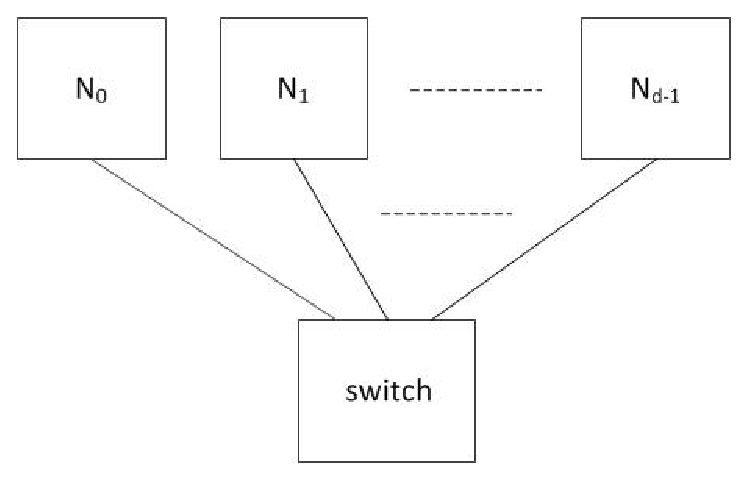
\includegraphics[width=0.4\textwidth]{distributed_system.eps}
\caption{The distributed system of $d$ computing nodes. }
\label{fig:distributed_system}
\end{figure}


\subsection{Details}

The algorithms lcpa-disk and lcpa-disk-m compute $ECP_{\log K}$ and $EPP_{\log K}$ via two runs of radix-sort in external memory. To emulate this radix-sort procedure in our distributed system, we set up a group of sending/receiding buffers in each computing nodes for data transmission during the sorts.

Algorithm~\ref{fig:alg:ds} shows our distributed algorithm lcpa-ds, where each round of the while-loop performs two runs of radix-sorts to compute the $fp$ field of each entry in $ECP_k$ and $EPP_k$ by using the sending and receiving buffers in lines~\ref{fig:alg:ds:s1}-\ref{fig:alg:ds:s2}. Specifically, for each entry $x$ in $ECP_{i,k}$, node $N_i$ dispatches $x$ to the sending buffer $SB1_{i,j}$ if $j = x.pos / e$ and delivers it to $RB1_{j,i}$ on $N_j$ in lines~\ref{fig:alg:ds:s1}-\ref{fig:alg:ds:s3}. Upon the arrival of each entry from the other nodes, $N_j$ caches the entry in its receiving buffers $\{RB1_{j,0},RB1_{j,1},...,RB1_{j,d-1}\}$ and then radix-sorts the received entries by $pos$ to form $IECP_{j,k}$ in lines \ref{fig:alg:ds:s4}-\ref{fig:alg:ds:s5}. Then it scans $T_j$ from left to right for iteratively computing the fingerprints of the involved prefix and record them in the $fp$ fields of the corresponding entries in $IECP_{j,k}$. Thereafter, in lines~\ref{fig:alg:ds:s6}-\ref{fig:alg:ds:s7}, each entry $y$ satisfying $i = y.pos /e$ is moved from $IECP_{j,k}$ to the sending buffer $SB1_{j,i}$ and then delivered to $RB1_{i,j}$ on $N_i$. Finally, $N_i$ radix-sorts the received entries in $\{RB1_{i,0},RB1_{i,1},...,RB1_{i,d-1}\}$ by their $idx$ to regenerate $ECP_{i,k}$ in lines~\ref{fig:alg:ds:s8}-\ref{fig:alg:ds:s2}. Note that the entries in $EPP_{i,k}$ can be processed using $\{SB2_{i,0}, SB2_{i,1},...,SB2_{i,d-1}\}$ and $\{RB2_{i,0}, RB2_{i,1}, ...,RB2_{i,d-1}\}$ in the same way as described above. Then, the algorithm generates $ECP_{i,k+1}$ and $EPP_{i,k+1}$ by scanning $ECP_{i,k}$ and $EPP_{i,k}$ once in line~\ref{fig:alg:ds:s9}.


\begin{algorithm}[t!]
\caption{Compute $K$-Order $LCPA_T[ie,ie+e)$ on $N_i$}
\label{fig:alg:ds}
lcpa-ds($T_i$, $SA_{T_i}$, $e$, $K$){\\
	\SetAlgoNoLine
	Scan $T_i$ rightward to compute $ECP_{i,0}$ and $EPP_{i,0}$. \\
	Let $k=0$. \\
	For $j\in[0,d)$, create sending buffers $SB1_{i,j}$ and $SB2_{i,j}$. \\
	For $j\in[0,d)$, create receiving buffers $RB1_{i,j}$ and $RB2_{i,j}$. \\
	\While{$k < \log K$}{
		\Indentp{-1em}
		For $j\in[0,d)$ and $p\in[0,2e)$, scan $ECP_{i,k}$ and $EPP_{i,k}$ rightward to cache $ECP_{i,k}[p]$ in $SB1_{i,j}$ or $EPP_{i,k}[p]$ in $SB2_{i,j}$ if $ECP_{i,k}[p].pos$ or $EPP_{i,k}[p].pos$ belongs to $[je,je+e)$. \label{fig:alg:ds:s1}\\
		For $j\in[0,d)$, send entries in $SB1_{i,j}$ and $SB2_{i,j}$ to $RB1_{j,i}$ and $RB2_{j,i}$ on $N_j$. \label{fig:alg:ds:s3}\\
		For $j\in[0,d)$, cache entries from $SB1_{j,i}$ and $SB2_{j,i}$ on $N_j$ in $RB1_{i,j}$ and $RB2_{i,j}$. \label{fig:alg:ds:s4}\\
		Radix-sort entries in $RB1_i$ and $RB2_i$ by $pos$ to produce $IECP_{i,k}$ and $IEPP_{i,k}$. \label{fig:alg:ds:s5}\\
		For $p\in[0,e)$ and $q\in [0,2e)$, scan $T_i$ rightward to iteratively compute the fingerprint of ${\sf pre}(T,ie+p)$ and assign ${\sf fp}(0,ie+p)$ to $IECP_{i,k}[q].fp$ or $IEPP_{i,k}[q].fp$ if $IECP_{i,k}[q].pos = ie+p$ or $IEPP_{i,k}[q].pos = ie+p$. \\
		For $j\in[0,d)$ and $p\in[0,2e)$, scan $IECP_i$ and $IEPP_i$ rightward to cache $IECP_{i,k}[p]$ in $SB1_{i,j}$ or $IEPP_{i,k}[p]$ in $SB2_{i,j}$ if $IECP_{i,k}[p].pos$ or $IEPP_{i,k}[p].pos$ belongs to $[je,je+e)$. \label{fig:alg:ds:s6}\\
		For $j\in[0,d)$, send entries in $SB1_{i,j}$ and $SB2_{i,j}$ to $RB1_{j,i}$ and $RB2_{j,i}$ on $N_j$. \label{fig:alg:ds:s7}\\
		For $j\in[0,d)$, cache entries from $SB1_{j,i}$ and $SB2_{j,i}$ on $N_j$ in $RB1_{i,j}$ and $RB2_{i,j}$. \label{fig:alg:ds:s8}\\
		Radix-sort entries in $RB1_i$ and $RB2_i$ by $idx$ to reproduce $ECP_{i,k}$ and $EPP_{i,k}$. \label{fig:alg:ds:s2}\\
		For $p\in [0,e)$, scan $ECP_{i,k}$ and $EPP_{i,k}$ rightward to compute and compare the fingerprints of $T[ECP_{i,k}[2p].pos+1, ECP_{i,k}[2p+1].pos]$ and $T[EPP_{i,k}[2p].pos+1, EPP_{i,k}[2p+1].pos]$ for generating $ECP_{i,k+1}$ and $EPP_{i,k+1}$. \label{fig:alg:ds:s9}\\
		Let $k=k+1$. \\
	}
	For $p\in [0,e)$, scan $T_i$, $ECP_{i,\log K}$ and $EPP_{i,\log K}$ rightward to literally compute $\Upsilon_{i,p}={\sf lcp}(ECP_{i,\log K}[2p].pos,EPP_{i,\log K}[2p].pos)$. \label{fig:alg:ds:s10}\\
	For $p\in [0,e)$, let ${\sf lcp}(SA_{T_i}[p],SA_{T,i}[p-1])=ECP_{i,\log K}[2p].pos + \Upsilon_{i,p} - SA_{T_i}[p]$. \label{fig:alg:ds:s11}\\
}
\end{algorithm}


After the while-loop, the steps in lines~\ref{fig:alg:ds:s10}-\ref{fig:alg:ds:s11} figure out the LCP-array of $T[ie,ie+e)$ in linear time from $ECP_{i,{\log K}}$, $EPP_{i,{\log K}}$ and $SA_{T_i}$ residing on $N_i$. Finally, we can simply collect and concatenate the LCP-array on each node to form $LCPA_T$. Hence, we get this result:

\begin{Lemma}
\label{thm:lcp:pdm}
Given $T$ and $SA_T$, the $K$-order $LCPA_T$ can be correctly computed in $\mathcal{O}(\frac{n}{d}\log K)$ time using $\mathcal{O}(\frac{n}{d})$ disk space on each computing node with a high probability.
\end{Lemma}
Proof. Algorithm~\ref{fig:alg:ds} exploits the use of sending/receiving buffers to perform the radix-sorts among the computing nodes in a distributed manner, where the overhead of time and space for data transmission sums up to $\mathcal{O}(e\log K)$ during the whole loop, for each node sends and receives $\mathcal{O}(e)$ entries per round.


It is noteworthy that the internal memory on each node is partitioned into two parts, where the first part maintains the sending/receiving buffers and the other part establishes the I/O buffers for reading/writing and sorting the entries of $ECP_{i,k}$ and $EPP_{i,k}$. High performance can be achieved if these buffers are large enough to compensate the delay of data transmission and amortize the overhead of each I/O operation.

\section{Experimental Results}\label{sec:experimental_results}

A series of simulation experiments are conducted on a real data set collected from the web site \url{http://download.wikimedia.org/enwiki/} for performance evaluation of our {C++} programs for the external and distributed algorithms presented in Section~\ref{sec:construction_in_em} and~\ref{sec:construction_in_distributed}, in terms of time and space consumption. We employ lcpa-disk-m as a baseline for performance and scalability assessment of lcpa-disk. The hardware platform for lcpa-disk and lcpa-disk-m is a computer equipped with 2 Intel Xeron E3-1220 CPUs, a 4GB DDR3 main memory and a 2TB 7200RPM disk, while the one for lcpa-ds is a distributed system consisting of 4 identical computers interconnected with a gigabit switch. We use gcc 4.8.4 and its MPI alternative~(mpicc) to compile the programs for lcpa-disk/lcpa-disk-m and lcpa-ds, respectively, under Ubuntu 14.04 operating system.

STXXL~\cite{Dementiev2007} is a {C++} STL library designed for efficient computations in external memory, freely available at \url{http://stxxl.sourceforge.net/}. Instead of to develop a radix sorter specific for our purpose, we use STXXL to perform the external memory sorts in our programs. Specifically, a priority queue  provided by STXXL is employed for sorting the entries in $ECP_k/EPP_k$ by $pos$ to form $IECP_k/IEPP_k$ and another for sorting them back by $idx$. Benefitting from the powerful priority queues, the programs for lcpa-disk, lcpa-disk-m and lcpa-ds are less than 400, 600 and 700 lines, respectively.

Each result in the following tables and figures is a mean of two runs of the programs, where the running time and peak disk use are collected by shell command ``time" and ``stxxl::block\_manager" provided by STXXL, respectively.

\subsection{Performance of the External Algorithms}

The following parameters and metrics are used for the experiments:
\begin{itemize}
\item $S$: corpora size.
\item $ST$: total running time.
\item $MT$: average running time spent in processing a character per loop's round.
\item $PD$: peak disk use.
\item $LR$: number of loop's rounds.
\item $W$: every $W$ successive loop's rounds in lcpa-disk are merged into one in lcpa-disk-m.
\item $H$: internal memory allocated to each priority queue when sorting the entries in external memory.
\end{itemize}

To show the effect of $W$, we demonstrate in Table \ref{tbl:disk_vs_diskm} the experimental results of lcpa-disk and lcpa-disk-m. As can be seen, lcpa-disk-m has a smaller $ST$ than lcpa-disk when $W=2$, while the latter outperforms the former in terms of $MT$ and $PD$. Specifically, given $K=8192$, the speed of lcpa-disk-m for $W=2$ is nearly 1/3 faster than that of lcpa-disk when $S$ varies from 200MB to 2GB. However, the total running time of lcpa-disk-m for $W=3$ grows rapidly as $S$ increases and exceeds that of lcpa-disk when $S$ approaches 2GB. This can be explained as follows. As described in Section~\ref{sec:construction_in_em}, lcpa-disk-m can merge every $W$ successive loop's rounds for decreasing $LR$ by computing all the fingerprints possibly involved in these $W$ successive loop rounds. For example, given $W=2$ and $W=3$, lcpa-disk-m maintains 3 and 7 fingerprints in each entry of $ECP_k$ and $EPP_k$, respectively, and updates them during each round of the loop. This leads to a sharp growth in the computation and I/O overhead per round against lcpa-disk and becomes a performance bottleneck.

Fig.~\ref{fig:disk_vs_diskm} illustrates the variation trend of $MT$ with increasing $S$. The non-linear relationship between the two parameters (i.e. $MT$ and $S$) violates the assumption that $MT$ is linear proportional to $S$. This behavior is partially due to the use of STXXL, where the priority queue provided by the library takes logarithmic time to sort elements in external memory.

\begin{table*}[htbp!]
	\begin{threeparttable}
		\caption{The performance results for the external memory algorithms.}
		\label{tbl:disk_vs_diskm}
		\centering
		\begin{tabular}{|c|c|c|c|c|c|c|c|c|c|c|c|c|}
			\hline
			$S$ & \multicolumn{4}{c|}{lcpa-disk} & \multicolumn{4}{c|}{lcpa-disk-m ($W = 2$)} & \multicolumn{4}{c|}{lcpa-disk-m ($W = 3$)}\\
			\cline{2-13}
			(MB) & $LR$ & $MT$ & $ST$ & $PD$ & $LR$ & $MT$ & $ST$ & $PD$ & $LR$ & $MT$ & $ST$ & $PD$\\
			\hline
			200 & 13 & 1.03 & 2803 & 30.94 & 7 & 1.33 & 1950 & 47.36 & 5 & 2.43 & 2541 & 77.52\\
			\hline
			400 & 13 & 1.11 & 6034 & 31.50 & 7 & 1.40 & 4108 & 47.36 & 5 & 2.20 & 4605 & 78.58\\
			\hline
			600 & 13 & 1.18 & 9650 & 31.58 & 7 & 1.48 & 6928 & 47.36 & 5 & 3.14 & 9860 & 130.86\\
			\hline
			800 & 13 & 1.34 & 14557 & 31.52 & 7 & 1.80 & 10547 & 47.38 & 5 & 3.06 & 12827 & 103.50\\
			\hline
			2048 & 13 & 1.72 & 48021 & 46.04 & 7 & 2.47 & 37029 & 60.48 & 5 & 4.59 & 49280 & 94.40\\
			\hline
		\end{tabular}
		\begin{tablenotes}
			\item Notes: $LR$, $MT$ in microseconds per (character $\cdot$ round), $ST$ in seconds and $PD$ in bytes per character, where $K=8192$, $W \in \{2,3\}$ and $S$ from 200MB to 2GB.
		\end{tablenotes}
	\end{threeparttable}
	\centering
\end{table*}

\begin{table*}[htbp!]
	\begin{threeparttable}
		\caption{The performance results for the distributed algorithm.}
		\label{tbl:diskm_vs_ds}
		\centering
		\begin{tabular}{|c|c|c|c|c|c|c|c|c|}
			\hline
			$S$ & $LR$ & \multicolumn{3}{c|}{lcpa-ds~($N=4$)} & \multicolumn{3}{c|}{lcpa-disk-m} & ST Ratio\\
			\cline{3-8}
			(MB) & & $MT$ & $ST$ & $PD$ & $MT$ & $ST$ & $PD$ & (\%)\\
			\hline
			200 & 7 & 0.71 & 1038 & 13.50 & 1.33 & 1950 & 47.36 & 0.54 \\
			\hline
			400 & 7 & 0.72 & 2113 & 13.50 & 1.40 & 4108 & 47.36 & 0.52 \\
			\hline
			600 & 7 & 0.74 & 3235 & 13.75 & 1.48 & 6928 & 47.36 & 0.50 \\
			\hline
			800 & 7 & 0.78 & 4547 & 13.82 & 1.80 & 10547 & 47.38 & 0.43 \\
			\hline
			2048 & 7 & 1.24 & 18617 & 16.21 & 2.47 & 37029 & 60.48 & 0.50 \\
			\hline
		\end{tabular}
		\begin{tablenotes}
			\item Notes: $LR$, $MT$ in microseconds per (character $\cdot$ round), $ST$ in seconds and $PD$ in bytes per character, where $K=8192$, $d=4$, $W=2$ and $S$ from 200MB to 2GB.
		\end{tablenotes}
	\end{threeparttable}
	\centering
\end{table*}

\begin{figure}[t]
\centering
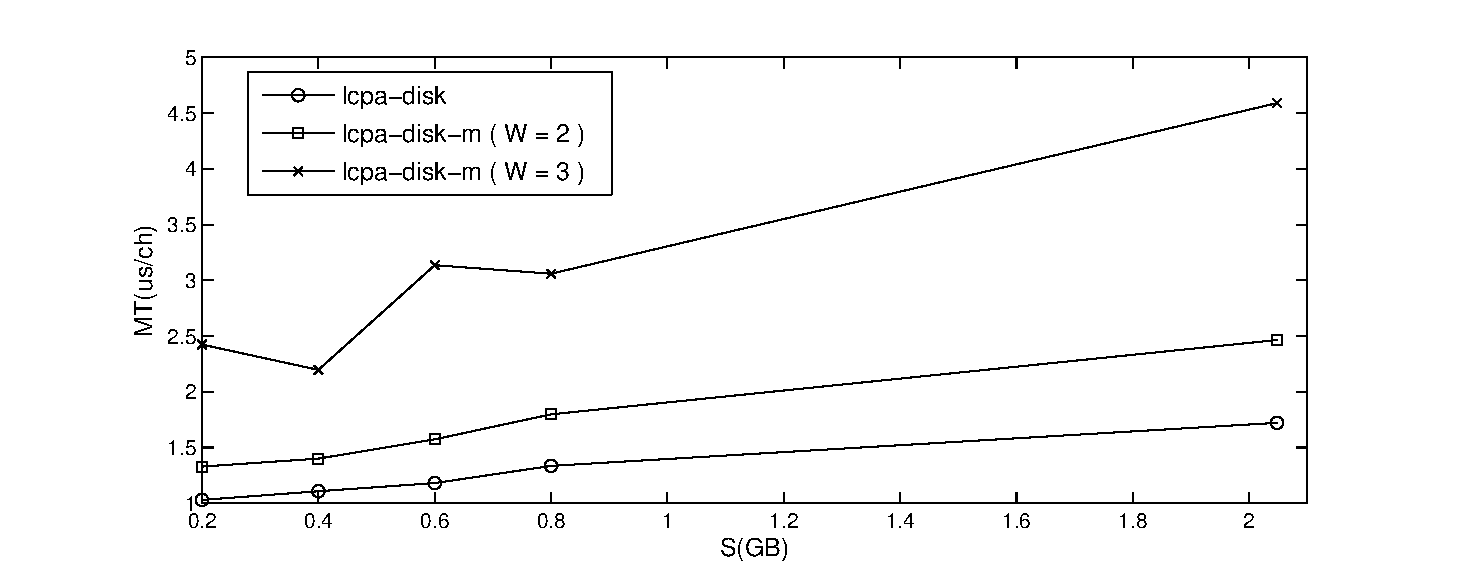
\includegraphics[width=1\textwidth]{disk_vs_diskm.eps}
\caption{$MT$ for lcpa-disk and lcpa-disk-m with $S$ varying from 200MB to 2GB, given $K=8192$ and $W\in \{2,3\}$.}
\label{fig:disk_vs_diskm}
\end{figure}

As reported in~\cite{Juha2014}, the disk space requirements for eSAIS and LCPscan are $65n$ and $21n$ bytes, respectively, while the peak disk use of our implementation for lcpa-disk-m~($W=2$) rises up to $61n$ bytes for processing a 2GB corpora. This indicates that {lcpa-disk-m} has a space requirement comparable to that of eSAIS, but around 3 times as that of  LCPscan. However, as will be seen in the following part, our method is much easier to be implemented and strongly scalable for the parallel and distributed model. In particular, the communication overhead on each node of the distributed model is balanced as $\mathcal{O}(\frac{n}{d})$. For $d\ge 3$, the space required by each node will be less than that of LCPscan.

\subsection{Performance of the Distributed Algorithm}

The algorithm lcpa-ds is strongly scalable, in terms of that it can be naturally executed in parallel except for the external memory sorts. We have described in Section~\ref{sec:construction_in_distributed} how to emulate the sorter by using a group of sending/receiving buffers. The communication overhead of each computing node in~Fig.~\ref{fig:distributed_system} is upper bounded by $\mathcal{O}(e)$. According to Amdahl's Law, the theoretical speed of lcpa-ds is $d-1$ times faster than that of lcpa-disk, where $d$ is the number of computing nodes in the distributed system. To validate this point, we adopt lcpa-disk-m as a baseline to evaluate the performance of lcpa-ds.

As observed from Table.~\ref{tbl:diskm_vs_ds}, given $K=8192$, $W=2$ and $d=4$, lcpa-ds outperforms lcpa-disk-m in terms of time and space consumption, where $MT/ST$ and $PD$ for the former are 1/2 and 1/4 times of that for the latter, respectively. Particularly, $MT$ for lcpa-ds increases from 0.71 to 1.24 when $S$ increases from 200MB to 2GB. However, the performance gain does not fully meet our expectation for the ideal case. The main reason lies on the limited internal memory capacity available on each computing node. In our implementation of the program, each computing node spends its internal memory on not only the sending/receiving buffers, but also the I/O buffers and internal memory heaps. Each internal memory heap is employed by a priority queue for amortizing the overhead of disk accesses when swapping data between the internal and external memory. The swapping process is fast when $H$ is large enough, because most of the data can be cached in the internal memory heap. However, a significant performance degradation in $MT$ will occur when $H$ becomes smaller, as shown in Fig.~\ref{fig:stxxl_pq_impact}. One solution for relieving the problem is to reduce the block size $e$ by adding more computing nodes. Fig.~\ref{fig:ds_varying_n} shows that, when $S$ increases from 200MB to 2GB, $MT$ is much smaller and grows more slowly for $d = 4$ against that for $d = 2$, due to a decrease in the overhead for I/O operations.


\begin{figure}[t]
\centering
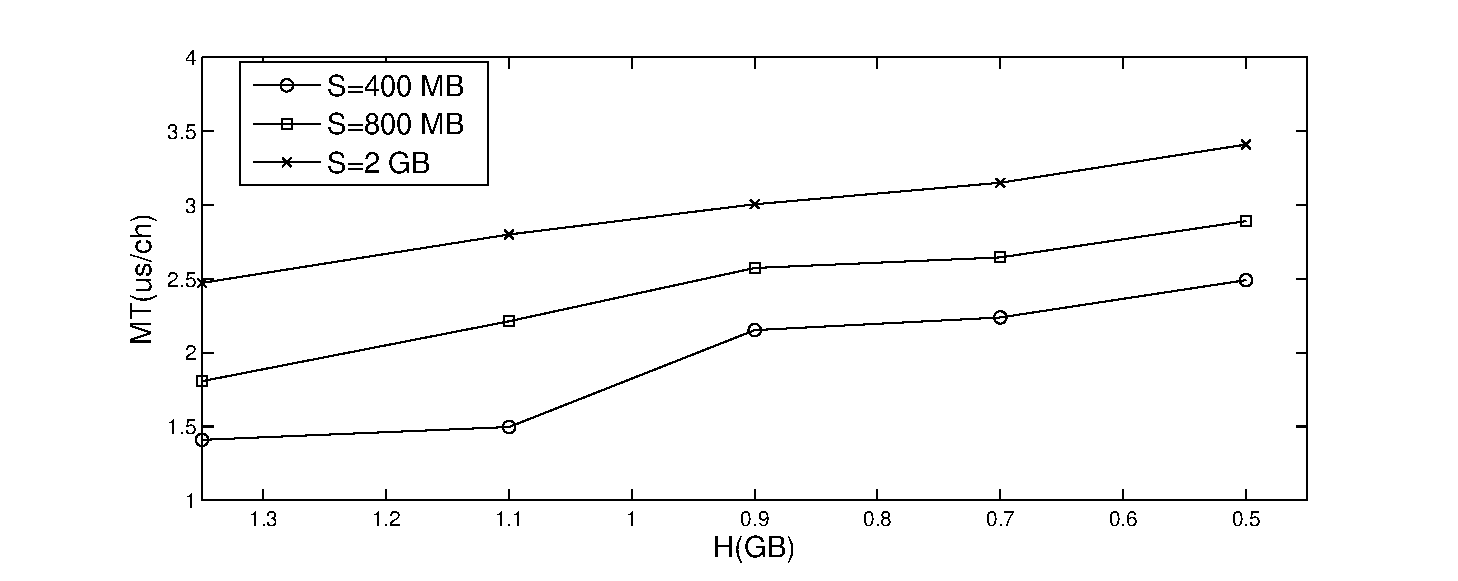
\includegraphics[width=1\textwidth]{stxxl_pq_impact.eps}\\
\caption{$MT$ for lcpa-disk-m with $H$ varying from 1.35 to 0.5GB, given $K=8192$, $W=2$, $d=4$ and $S \in \{400, 800, 2048\}$ MB.}
\label{fig:stxxl_pq_impact}
\end{figure}



\begin{figure}[t]
\centering
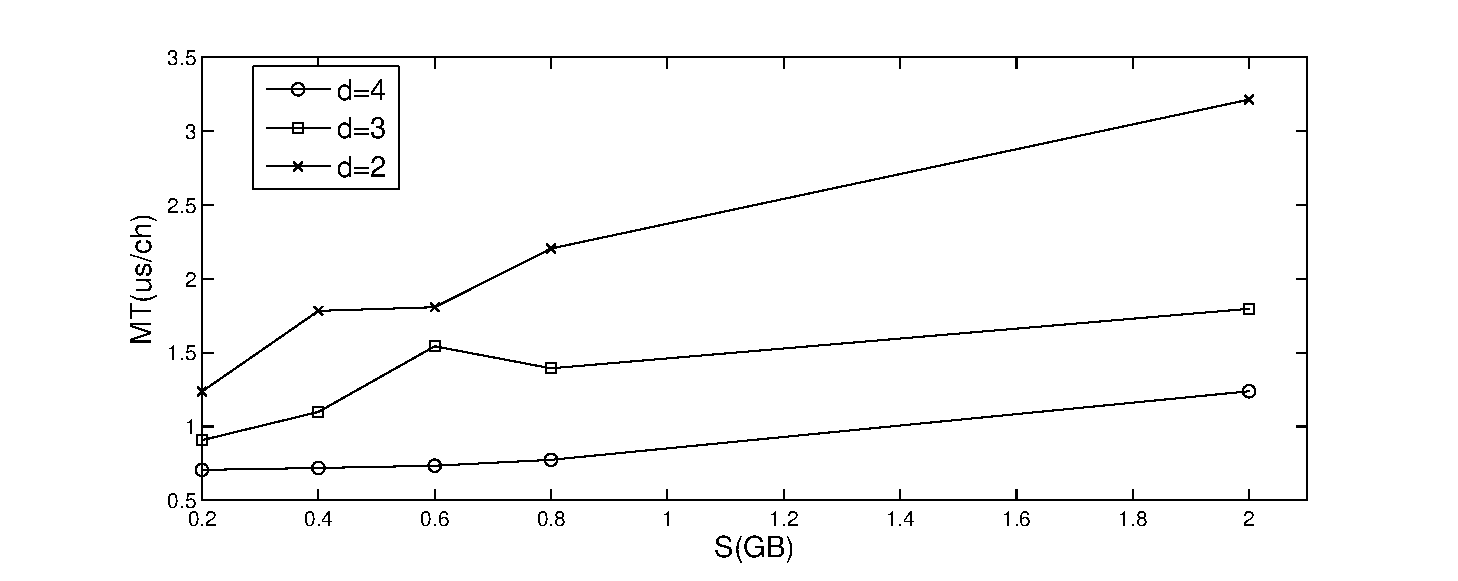
\includegraphics[width=1\textwidth]{ds_varying_n.eps}\\
\caption{$MT$ for lcpa-ds with $S$ varying from 200MB to 2GB, given $K=8192$, $W=2$ and $d \in \{2,3,4\}$.}
\label{fig:ds_varying_n}
\end{figure}


\section{Conclusion}\label{sec:conclusion}

We present in this paper a practical $K$-order LCP-array construction method that can be easily applied on both the internal memory and the external memory models. The program for lcpa-disk-m is less than 600 lines when using STXXL to implement the external sorts. We also show that the proposed method is straightforward to be extended for running on a typical distributed system of a cluster of $d$ computing nodes, where the time and space complexities are evenly divided onto each node as $\mathcal{O}(\frac{n}{d}\log K)$ and $\mathcal{O}(\frac{n}{d})$, respectively. The proposed algorithms are simple in design and universal for the internal memory, external memory and distributed models. Its implementations on all these models are not difficult and easily to be deployed.
A cluster of computers in a local area network are commonly available in practice, but there is currently a lack of scalable LCP-array construction algorithms for such a distributed model. In this sense, our algorithms provide a candidate solution to meet the demand. For performance improvement of the algorithms, we are investigating techniques to exploit the use of GPUs for speeding up the computation of fingerprints.

\section*{Acknowledgment}
The work of G. Nong was supported by the Guangzhou Science and Technology Program grant 201707010165 and the Project of DEGP grant 2014KTSCX007. The work of W. H. Chan was supported by GRF (18300215), Research Grant Council, Hong Kong SAR.

\bibliographystyle{unsrt}
\bibliography{bibfile}

\end{document}
